\documentclass[12pt]{report}
\usepackage{lmodern}
\usepackage[T1]{fontenc}
\usepackage{graphicx} % Allows you to insert figures
\usepackage{amsmath} % Allows you to do equations
\usepackage{fancyhdr} % Formats the header
\usepackage{geometry} % Formats the paper size, orientation, and margins
\usepackage[style=numeric,backend=biber,citestyle=numeric-comp,sorting=none,maxbibnames=99,giveninits=true,doi=true,isbn=false,url=false]{biblatex} 

\usepackage[colorlinks=true, linkcolor=black, citecolor=black, urlcolor=black]{hyperref}
\usepackage{booktabs}
\usepackage[version=4]{mhchem}
\usepackage{listings} % For code
\usepackage{float}
\usepackage{subcaption}
\usepackage{wrapfig}
\usepackage[format=plain, font=it]{caption} % Italicizes figure captions
\usepackage[english]{babel}
\usepackage{csquotes}
\usepackage{titlesec}

\AtEveryBibitem{
    \clearfield{urlyear}
    \clearfield{urlmonth}
    \clearfield{month}
    \clearlist{language}
} % Removes access date, months, and language from bibliography

\renewbibmacro{in:}{} % Removes the "In" before journal names

% Removed Harvard-specific settings and unnecessary macros:
% \citetrackerfalse % Not needed for numeric citations
% \DeclareNameAlias{sortname}{family-given} % Optional for Vancouver style, removed

% Vancouver-style superscript citations
\addbibresource{references.bib} % Specifies the bibliography file
\DeclareFieldFormat{labelnumber}{#1}
\renewcommand{\bibopenbracket}{}
\renewcommand{\bibclosebracket}{}
\renewcommand{\cite}{\supercite}
\renewcommand{\bibname}{References}
\DefineBibliographyStrings{english}{
  bibliography = {References}\textbf{}}

% Command to simplify images
\newcommand{\addimage}[4][0.8]{
    \begin{figure}[h]
        \centering
        \includegraphics[width=#1\linewidth]{Images/#2}
        \caption{#3}\label{fig:#4}
    \end{figure}
} % \simpleimage[ratio of linewidth (i.e. 0.5)]{image_name}{caption}{reference_name}

% Paper Properties
\linespread{1.15} % about 1.5 spacing in Word
\setlength{\parindent}{0pt} % no paragraph indents
\setlength{\parskip}{0.5em} % paragraphs separated by one line
\urlstyle{same} % makes a nicer URL and DOI font
\renewcommand{\headrulewidth}{0pt}
\geometry{letterpaper, portrait, margin=1in}
\setlength{\headheight}{14.49998pt}

% Title Formats
\titleformat{\chapter}[block]{\normalfont\large\bfseries\centering}{\thesection}{0.5em}{}
\titlespacing*{\chapter}{0pt}{0em}{0.5em}
\titleformat{\section}[block]{\normalfont\large\bfseries}{\thesection}{0.25em}{\vspace{-0.5em}}
\titleformat{\subsection}[block]{\normalfont\normalfont\bfseries}{\thesubsection}{0.25em}{\vspace{-0.25em}}
\titleformat{\subsubsection}[block]{\normalfont\normalfont\bfseries\itshape}{\thesubsubsection}{0.25em}{\vspace{-0.25em}}
% Remove chapter number from headings (due to report class)
\setcounter{secnumdepth}{3}
\setcounter{section}{0}
\renewcommand{\thesection}{\arabic{section}.}
\renewcommand{\thesubsection}{\arabic{section}.\arabic{subsection}.}
\renewcommand{\thesubsubsection}{\arabic{section}.\arabic{subsection}.\arabic{subsubsection}.}

\raggedright % Removes justification completely
%\sloppy % Make the right edge sloppy, use \fussy to change back

\newcommand\titleofdoc{Non-intrusive Testing of Liquid Culture Medium using Online NIR Spectroscopy and Machine Learning for Qualitative Analysis} %%%%% Put your document title in this argument

\begin{document}
\begin{titlepage}
   \begin{center}
        \vspace*{2.5cm} % Adjust spacings to ensure the title page is generally filled with text

        \Large{\bfseries{\titleofdoc}} 

        \vspace{0.5cm}
            
        \vspace{3cm}
       
        \vspace{0.25cm}
        \large{Connor Reintjes, Paola Gonz\'alez P\'erez, Benjamin Samuel, Shiza Hassan}

        \vspace{0.25cm}
        \large{Supervisor: Dr. Amin Reza Rajabzadeh}
       
        \vspace{3 cm}
        \large{McMaster University, W. Booth School of Engineering Practice and Technology}
        
        \vspace{0.25 cm}
        \large{BIOTECH 4TR3 - Capstone}
       

       \vfill
    \end{center}
\end{titlepage}

\setcounter{page}{2}
\pagestyle{fancy}
\fancyhf{}
\rhead{\thepage}
\lhead{Reintjes, Gonz\'alez P\'erez, Samuel, Hassan}

\chapter*{Abstract}
Insufficient quality assurance is a major expense associated with laboratories that can result in contamination, poor sample integrity, and lead to lost time due to repetitive sample testing. To ameliorate these issues, NIR spectroscopy has been combined with machine learning in this approach to qualitatively analyze the composition of liquid cultures in a non-intrusive and online manner. This will allow laboratories to save time by identifying contamination as soon as it happens and proceeding accordingly, as opposed to finding out after a full protocol has been performed. The method to achieve this involved creating a casing to house the NIR which would take spectra of the sample and pass it to a machine learning model that would then identify whether the sample is in a normal or contaminated state. In phase 1 of the experiment, the NIR housing was manufactured and initial testing was conducted for both contaminated and non-contaminated states, with the contaminant being Lactobacillus rhamnosus. The results achieved indicate that the NIR was able to differentiate between contaminated and non-contaminated samples. In phase 2, further data collection was conducted using a quartz cuvette and Teflon background to reduce noise and spectra interference. A data augmentation pipeline was constructed to overcome data size limitations. The processed data was then fed into a 1D-CNN model to obtain preliminary results on its performance. Implementation of one-class classification resulted in the overfitting of the model. The pipeline and 1D-CNN model will continue to be developed in order to improve their performance as more diverse data is collected.

\thispagestyle{empty}

\newpage
\tableofcontents
\thispagestyle{empty}
\newpage

\section{Introduction} % If you want numbered sections, remove the star after \section

Quality assurance issues are responsible for repeated testing, misdiagnosis, improper treatment and unpredictable costs.\cite{CostPoorQualityrandoxlaboratories} The contamination of samples is the most common problem experienced in microbial laboratories. The real-time monitoring of samples can represent a significant cost-saving solution to improve quality assurance practices in laboratory and industrial settings.\cite{ContaminationMicrobiologicalLaboratoryendeshawabatenh2018} To improve these issues, Near Infrared (NIR) spectroscopy has been combined with deep learning to provide real-time analysis of sample quality. This online analysis increases the testing and result obtention speed while remaining non-invasive to reduce further contamination of the samples.\cite{SpeechRecognitionUsingalsobhani2021} This technology also symbolizes a financial advantage by reducing the loss of biological samples using low computational requirements that can measure and classify the analyzed data as required. A deep learning model will be used to optimize this analysis as it offers advantages such as automatically integrating feature extraction, and incorporating hundreds of layers with many parameters compared to artificial neural networks.\cite{DeepLearningNearinfraredmishra2022}

The NIR spectral region has a range from 700 nm to 2500 nm. It is primarily characterized by absorption bands corresponding to the overtone and combination bands of \ce{C-H}, \ce{N-H}, \ce{O-H}, and \ce{S-H} stretching \autoref{fig:principle_bands}. Hence, the spectra of most compounds will show unique absorption peaks in the NIR spectral region. These peaks can be used for the quantitative and qualitative analysis of the compounds in gases, solids or liquids.

\begin{figure}[h]
    \centering
    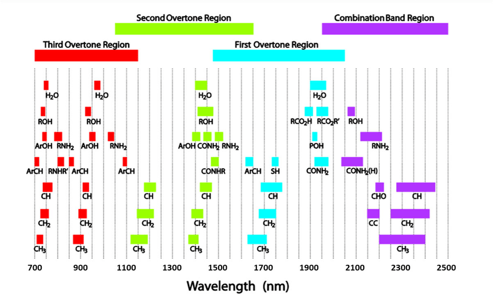
\includegraphics[width=0.75\linewidth]{Images/principle_bands.png}
    \caption{Principal analytical bands and relative peak locations for absorptions in the near-infrared region.\emph{NEEDS CITATION} Unique absorptions found in the majority of chemical and biological products can be utilized in both qualitative and quantitative examinations.}
    \label{fig:principle_bands}
\end{figure}

Ethanol and water have characteristic NIR spectrum patterns that allow for their identification and quantification as seen in \autoref{fig:anton_paar}. Ethanol has a unique narrow peak at $1200$ nm representing the second overtone of the \ce{C-H} stretching vibration.\cite{InfraredSpectroscopyNIR} Water, on the other hand, shows a flat behaviour at this wavelength due to the lack of \ce{C-H} bonds. 

The intensity of NIR absorption bands is $10-100$ times lower than that of the equivalent basic mid-IR absorption bands. This facilitates the direct analysis of strong absorbances and high light-scattering efficiency. Band overlap and penetration depth reduce in the near-infrared (NIR) spectral region, whereas the efficiency of light scattering and absorptivity improves with wavelength. As NIR spectroscopy depends on light absorption, spectral data can be acquired either in transmittance or reflectance mode. Diffuse reflectance $(\log \frac{1}{R} )$ measurements are favored for opaque or light-scattering matrices whereas translucent samples used transmittance $(\log \frac{1}{R})$.

\begin{wrapfigure}{r}{0.5\textwidth}
    \centering
    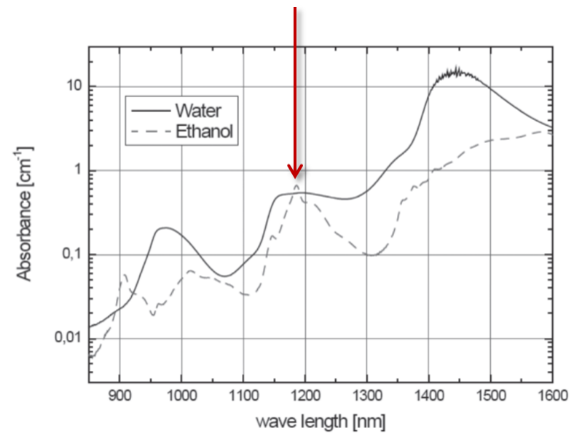
\includegraphics[width=0.48\textwidth]{Images/anton_paar.png}
    \caption{NIR spectrum of ethanol and water \cite{InfraredSpectroscopyNIR}}
    \label{fig:anton_paar}
\end{wrapfigure}

NIR spectroscopy's quickness, adaptability to a variety of materials, and capacity to examine liquid samples make it a promising tool for bio applications.\cite{NearInfraredSpectroscopyBioApplicationsbec2020} Recent advancements are making NIR spectroscopy more accessible with portable handheld instruments that allow for real-time, on-site examination. 
Cell culture media (CCM) plays a vital role, directly impacting process yield and product quality.\cite{CellCultureMediaryder2018} CCM's primary objective is to create and sustain an optimal physiological environment for large-scale cell culturing, ensuring cell health and expression of desired Critical Quality Attributes (CQAs). However, it's crucial to recognize that the chemical and physical properties of CCM are sensitive to microbial growth, chemical reactions, and environmental factors like temperature and light. Without sterilization, CCM can rapidly change due to microbial contamination, leading to increased turbidity and light scatter, consequently elevating baselines and noise in spectra, potentially compromising measurements. While chemometrics can mitigate some measurement errors, identifying errors induced by samples and measurements in CCM analysis can be challenging.

NIR spectra are known to be high-dimensional data due to the baseline drift and other noise signals present. This results in the need for preprocessing techniques for noise filtering and dimensionality reduction before analyzing the true compound signals.\cite{1DConvolutionalNeuralkrohling2023} Hence,  NIR spectra usually involve the use of chemometric algorithms like partial least squares regression (PLSR) and support vector regression (SVR) to clean the data from baseline drift as well as to understand the chemical changes in the samples.\cite{NIRSpectroscopyCombinedshang2023,LinearSupportVectornaguib2014} These algorithms require trained individuals to obtain the necessary parameters used to analyze the spectra.\cite{QuantitativeAnalysisYeastwang2017} Similarly, chemometric models are often limited by their inability to generalize for variance in spectra from different instruments, or changing storage and growing conditions. Deep Learning\cite{ReviewEvolutionChemometricswalsh2023} Machine Learning (ML) can be used to automate extracting the main compound features from high-dimensional spectral data and eliminate the need for feature-selection techniques. 
While different classes of ML algorithms have successfully achieved the classification of NIR spectra,\cite{1DConvolutionalNeuralkrohling2023} traditional ML methods such as partial least squares (PLS), K-nearest neighbor (KNN), and principal component analysis (PCA) require a higher level of expertise to design suitable features of the models architecture.\cite{zhangReviewMachineLearning2022} Deep learning, on the other hand, does not require a high level of expertise as it utilizes the raw features of data to analyze and classify it as needed. This is achieved through multiple hidden layers that are trained end to end. Some of these layers can be specialized convolution layers that allow for the learning and identification of local feature patterns. This aspect enables deep learning architectures to employ less preprocessing for high-dimensional data.\cite{FastDeepLearningyue2021} 

Convolutional neural networks (CNNs) are a class of deep neural networks commonly used for data analysis due to their successful results in image processing and classification,\cite{AnalysisConvolutionalNeuralsharma2018} speech recognition,\cite{SpeechRecognitionUsingalsobhani2021} and other computer vision tasks. CNNs are a feed-forward multi-layer architecture in which a kernel or filter takes specific features from local regions from the upper layer.  This architecture allows for an autonomous extraction of important features from complex data for analysis and learning.\cite{NIRSpectroscopyCombinedshang2023} A common drawback of the use of CNNs for spectral analysis is the requirement of large data sets during the training process of the model.\cite{zhangNearInfraredSpectralCharacteristic2022} To avoid overfitting due to a limited number of data samples, one-dimensional CNN (1D-CNN) can be used. These models are similar to traditional CNNs except for the data size required and low computational requirements. 1D-CNNs have proven to have good information extraction and high classification accuracy with simple preprocessing techniques. It has been applied by Shang et al.\cite{NIRSpectroscopyCombinedshang2023} for the analysis and classification of NIR spectra from breast cancer tissue to aid in cancer diagnosis, demonstrating a $94.67\%$ classification accuracy. Chai et al.\cite{Improved1DConvolutionalchai2021} also developed an improved 1D-CNN structure to discriminate Anoectochilus roxburghii from its counterfeits using NIR spectra.
Previous studies performed on 1D-CNN for the analysis of NIR spectral data demonstrate the viability of its application for the online analysis of culture media. The present study aims to develop a method based on NIR spectra acquired on a portable device, as a non-destructive, online method to assess quality attributes of culture media. Due to the expected nature of the data collection, it was necessary to employ a time series analysis when designing the CNN structure. Within this experiment \emph{S. cerevisiae} was used as the model, testing it under two conditions, normal and contaminated with Lactic Acid Bacteria. \emph{Lactobacillus rhamnosus} was used as the contaminant of choice due to its improved growth in the presence of \emph{S. cerevisiae}. Also, using this species ensures the proper growth of \emph{S. cerevisiae} as it remains unaffected in its presence.\cite{YeastHumanCoevolutionnenciarini2024} The NIR spectra of ethanol were analyzed in each case and passed to the deep learning model which classified the “normal” baseline against a “non-normal” sample. 


\begin{wrapfigure}{r}{0.4\textwidth}
    \centering
    \includegraphics[width=0.38\textwidth]{example-image}
    \caption{A wrapped figure with forced placement.}
\end{wrapfigure}

Nullam quis cursus risus. Nullam vitae ligula non felis faucibus molestie. Praesent aliquam sed neque id dignissim. Morbi in lectus elementum, luctus purus eget, tempus metus. Maecenas ut blandit justo. Proin nisi nisi, pretium quis elit non, scelerisque fringilla mauris. Praesent vel velit neque. Vestibulum viverra ipsum vel lorem pellentesque, a consequat nisi vehicula. Nulla facilisi. Cras euismod, turpis sed vestibulum interdum, odio diam fringilla neque, eget auctor nunc erat quis tellus. In lobortis nunc elit, quis condimentum magna ultrices ut. Donec ipsum elit, volutpat eget enim at, venenatis egestas augue. Nam elementum ipsum in felis tristique pretium.

Etiam a mi cursus, vehicula magna id, vestibulum urna. Vivamus pharetra arcu tellus, eu dignissim felis suscipit ut. Phasellus et ligula aliquam, convallis elit quis, ullamcorper purus. Etiam turpis ligula, tincidunt sed tincidunt nec, pellentesque nec est. Fusce non mollis mi. Mauris ut elit tempor, euismod erat nec, lacinia metus. Morbi maximus neque dolor, nec pulvinar dui scelerisque et. Vestibulum efficitur mollis lobortis. In hac habitasse platea dictumst. Vestibulum ut nibh et felis scelerisque mattis a at mauris. Aliquam erat volutpat. Vivamus vel massa egestas, tempor dolor ac, imperdiet ipsum.

\section{Major Heading}
\subsection{Subheading}
\subsubsection{Subsubheading}
Etiam nec malesuada ex. Vestibulum laoreet purus nec metus egestas, sit amet fringilla ipsum laoreet. Pellentesque ornare, neque in convallis maximus, quam mi facilisis felis, sed cursus dui lectus sit amet felis. Proin finibus quis urna ut sollicitudin. Vestibulum congue, ex vitae suscipit efficitur, elit quam ullamcorper est, eget tempus mi velit eget mi. Integer eget nunc eu eros cursus bibendum. Vestibulum ultrices ligula quis nulla porta malesuada. Morbi vel mi vel erat tempor consectetur sed a arcu. Phasellus convallis nibh ut erat posuere, a pharetra ipsum viverra. Praesent scelerisque maximus urna. Nam mattis ac massa in scelerisque. Praesent vulputate feugiat diam id eleifend. Phasellus iaculis ut lectus vestibulum volutpat.

\begin{equation} % add * after equation for unnumbered equations
     \hat{H} \psi = i \hbar \frac{\partial \Psi}{\partial t}
\end{equation}

\begin{align} % good for multi-line equations. Alternatively use gather which centers equations
     \frac{D}{D_0} &= e^{-\frac{\mu}{\rho}\rho x} \\
    ln\left(\frac{D}{D_0}\right) &= -\frac{\mu}{\rho}\rho x \\
    x &= \frac{-ln\left(\frac{D}{D_0}\right)}{\frac{\mu}{\rho}\rho}
\end{align}
Lorem ipsum dolor sit amet, consectetur adipiscing elit. Sed blandit tortor ut pharetra auctor. Curabitur posuere massa vitae commodo malesuada. Lorem ipsum dolor sit amet, consectetur adipiscing elit. Ut aliquet lacus nec quam auctor, eget suscipit turpis efficitur. Sed convallis sed enim eu sagittis. Nunc pretium id lacus ut lacinia. Praesent gravida varius faucibus. Maecenas commodo pretium dignissim.

Nulla vulputate congue felis eget scelerisque. Aenean gravida scelerisque risus, id placerat magna condimentum quis. Proin in aliquet mi. Aenean accumsan luctus malesuada. Nam volutpat volutpat sapien. Praesent vitae finibus arcu. Sed blandit eu ex non condimentum. Maecenas lacus ligula, eleifend in elit non, fermentum ultrices turpis. Morbi viverra, dolor ultrices elementum convallis, enim magna pharetra mi, sit amet molestie magna urna vel risus. Maecenas at sem leo. Nunc vulputate nisi nec commodo malesuada. Donec iaculis cursus pulvinar. Curabitur sem quam, venenatis egestas lobortis sit amet, semper a sem. Donec enim nibh, interdum at libero ut, mattis sollicitudin lectus. Duis malesuada, odio et dictum scelerisque, felis ante tristique tellus, vel suscipit mi massa suscipit nisl. Suspendisse ullamcorper enim vel nisl porttitor, non placerat ipsum maximus.

\addimage[0.7]{Black Hole Image.jpg}{An Image of a Black Hole\cite{hawking_particle_1993}}{black_hole}

\section{Major Heading}
Etiam a mi cursus, vehicula magna id, vestibulum urna. Vivamus pharetra arcu tellus, eu dignissim felis suscipit ut. Phasellus et ligula aliquam, convallis elit quis, ullamcorper purus. Etiam turpis ligula, tincidunt sed tincidunt nec, pellentesque nec est. Fusce non mollis mi. Mauris ut elit tempor, euismod erat nec, lacinia metus. Morbi maximus neque dolor, nec pulvinar dui scelerisque et. Vestibulum efficitur mollis lobortis. In hac habitasse platea dictumst. Vestibulum ut nibh et felis scelerisque mattis a at mauris. Aliquam erat volutpat. Vivamus vel massa egestas, tempor dolor ac, imperdiet ipsum \cite{rojas_engadget_2006}.

Etiam nec malesuada ex. Vestibulum laoreet purus nec metus egestas, sit amet fringilla ipsum laoreet. Pellentesque ornare, neque in convallis maximus, quam mi facilisis felis, sed cursus dui lectus sit amet felis. Proin finibus quis urna ut sollicitudin. Vestibulum congue, ex vitae suscipit efficitur, elit quam ullamcorper est, eget tempus mi velit eget mi. Integer eget nunc eu eros cursus bibendum. Vestibulum ultrices ligula quis nulla porta malesuada. Morbi vel mi vel erat tempor consectetur sed a arcu. Phasellus convallis nibh ut erat posuere, a pharetra ipsum viverra. Praesent vulputate feugiat diam id eleifend. Phasellus iaculis ut lectus vestibulum volutpat \cite{amjad_value_2020}.

\newpage
\printbibliography % If something looks strange in the bibliography, more often than not, you can modify the parameter in the .bib to fix the problem
\thispagestyle{empty}

\appendix
\end{document}
